% Created 2016-03-01 Tue 15:09
\documentclass[11pt]{article}
\usepackage[utf8]{inputenc}
\usepackage{lmodern}
\usepackage[T1]{fontenc}
\usepackage{fixltx2e}
\usepackage{graphicx}
\usepackage{longtable}
\usepackage{float}
\usepackage{wrapfig}
\usepackage{rotating}
\usepackage[normalem]{ulem}
\usepackage{amsmath}
\usepackage{textcomp}
\usepackage{marvosym}
\usepackage{wasysym}
\usepackage{amssymb}
\usepackage{amsmath}
\usepackage[version=3]{mhchem}
\usepackage{url}
\usepackage{underscore}
\usepackage{threeparttable}
\usepackage{tabulary}
\usepackage{parnotes}
\usepackage{comment}
\usepackage{multirow}
\usepackage{booktabs}
\usepackage[innermargin=0.5in,outermargin=0.5in,vmargin=0.5in]{geometry}
\usepackage[dvipsnames,svgnames,table]{xcolor}
\usepackage[linktocpage,pdfstartview=FitH,colorlinks,linkcolor=blue,anchorcolor=blue,citecolor=blue,filecolor=blue,menucolor=blue,urlcolor=blue,citebordercolor={0 1 0}]{hyperref}
\usepackage{attachfile}
\author{David R. Hill and Shrikar Thodla}
\date{\today}
\title{SeqRetriever}
\hypersetup{
  pdfkeywords={},
  pdfsubject={},
  pdfcreator={Emacs 24.5.1 (Org mode 8.2.10)}}
\begin{document}

\maketitle
\tableofcontents

\section{Aims}
\label{sec-1}
High throughput RNA sequencing is an incredibly powerful tool for characterizing gene expression events ranging in scale from the complete transcriptome of an organism or tissue to the expression of a single rare RNA isoform accounting for the tiniest fraction of all trancriptional activity in a cell.  

SeqRetriever is designed to extract gene abundance data from the raw output of the \href{http://cole-trapnell-lab.github.io/cufflinks/}{Tophat/Cufflinks} transcriptome assembly and abundance estimation suite and convert it into R dataframes, commonly used plots, and universal CSV output files. This allows you to ask simple questions about differences in gene expression and generate output that you can share with your colleagues, advisors, collaborators, and reviewers without requiring a degree in computer science or lengthy immersion in boring programming blogs. We get it - you have papers that needed to be written yesterday and you don't have time to learn to program. We're even okay with you analyzing these output files in Excel if you want.

There are a variety of tools available for analyzing RNA-seq datasets in the R environment, including the outstanding \href{http://compbio.mit.edu/cummeRbund/}{CummeRbund} package designed for analyzing Cufflinks output which we highly recommend. SeqRetriever has far fewer features, focusing exclusively on differential expression analysis of assembled RNA-seq datasets. SeqRetriever aims to be the first R package you run to answer a brand new question about gene expression differences, but probably not the last one. This package is designed to get you asking, answering, refining, and re-asking your questions as quickly as possible.

\section{Design criteria}
\label{sec-2}
All functions in the SeqRetriever package are designed with the following criteria in mind:

\begin{enumerate}
\item Approachable - Anyone can generate meaningful, high quality data from RNA-seq datasets.
\item Productive - Functions should be simple and intuitive. You shouldn't have to pull up ?SeqDataframe in every R session. SeqRetriever functions should free your mind to think about science, not programming.
\item Readable - Good R script is easy to follow and, therefore, easier to share and debug. While discrete functions in SeqRetriever can be sequenced together in a pipeline to perform complex tasks, the induvidual SeqRetriever functions perform simple tasks and can be used independently of other SeqRetriever functions.
\end{enumerate}

\section{Work flow}
\label{sec-3}
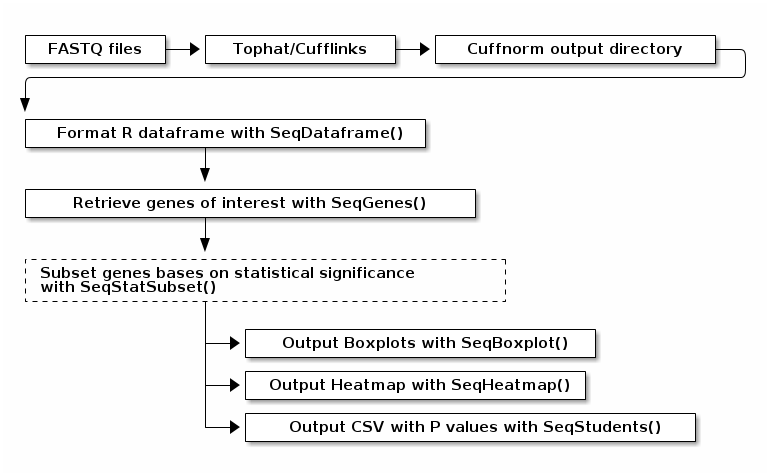
\includegraphics[width=.9\linewidth]{workflow.png}



\section{Examples}
\label{sec-4}

\subsection{Setup database}
\label{sec-4-1}
\begin{verbatim}
library(SeqRetriever)
getSRexample() # Downloads and unpacks example dataset in working directory
testdf <- SeqDataframe(dir = "./norm_out") # format dataframe
\end{verbatim}
\subsection{Select genes}
\label{sec-4-2}
\begin{verbatim}
genes <- SeqGenes(gene.names = c("OR4F5","SAMD11","AJAP1","SKI","ESPN", "CNKSR1"), df = testdf)
\end{verbatim}

\subsection{Print boxplot}
\label{sec-4-3}
\begin{verbatim}
plot <- SeqBoxplot(genes)
print(plot)
\end{verbatim}

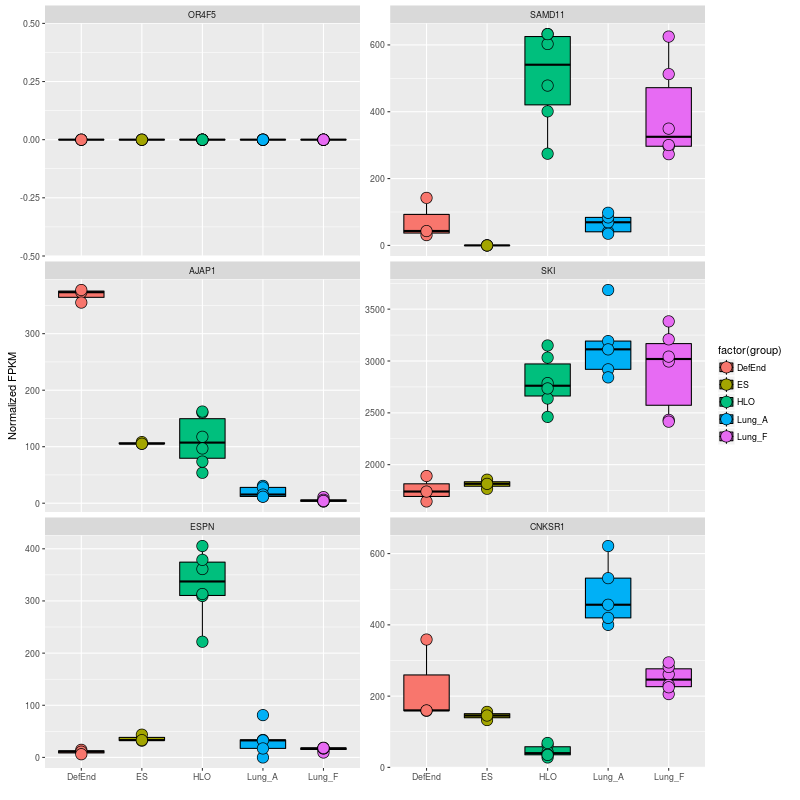
\includegraphics[width=.9\linewidth]{boxplots.png}
\subsection{Print Heatmap}
\label{sec-4-4}
\begin{verbatim}
SeqHeatmap(genes, hm.name = "heatmap.png")
\end{verbatim}

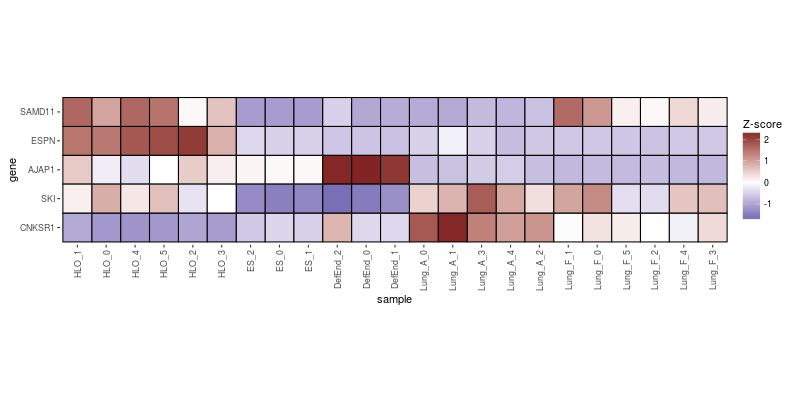
\includegraphics[width=.9\linewidth]{heatmap.png}

\subsection{Print boxplot showing only genes that differ significantly between "HLO" and "Lung$_{\text{A}}$"}
\label{sec-4-5}
\begin{verbatim}
sig.genes <- SeqStatSubset(genes, limit = 0.001, group1 = "HLO", group2 = "Lung_A")
plot2 <- SeqBoxplot(sig.genes, nrow = 1)
print(plot2)
\end{verbatim}

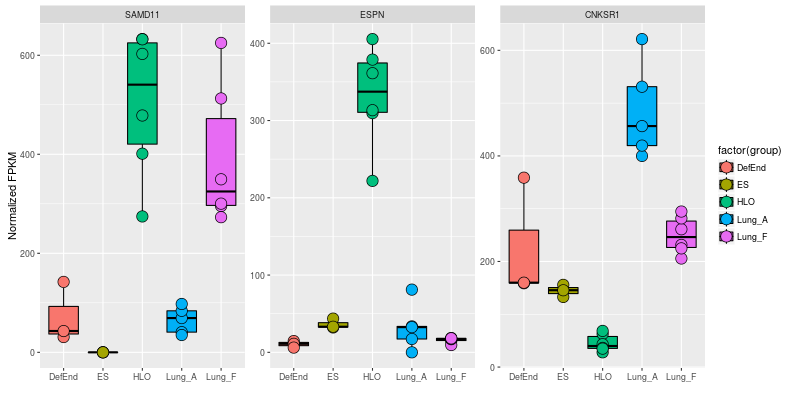
\includegraphics[width=.9\linewidth]{sig-boxplots.png}

\section{{\bfseries\sffamily } Install from Github}
\label{sec-5}
\begin{verbatim}
library(devtools)
devtools::install_github("hilldr/SeqRetriever/SeqRetriever")
\end{verbatim}
% Emacs 24.5.1 (Org mode 8.2.10)
\end{document}
